\documentclass[]{beamer}
% Class options include: notes, notesonly, handout, trans,
%                        hidesubsections, shadesubsections,
%                        inrow, blue, red, grey, brown

% Theme for beamer presentation.
\usepackage{beamerthemesplit} 



%%%%%%%%%%%%%%%%%%%%%%%%%%%%%%%%%%%%%%%%%%%%%%%%%%%%%%%%%%%%%%%%%%%%%%



\definecolor{mypink1}{rgb}{0.858, 0.188, 0.478}

\newcommand{\mybox}{%
    \collectbox{%
        \setlength{\fboxsep}{1pt}%
        \fbox{\BOXCONTENT}%
    }%
}

%%%%%%%%%%%%%%%%%%%%%%%%%%%%%%%%%%%%%%%%%%%%%%%%%%%%%%%%%%%%%%%%%%%%%%
% Other themes include: beamerthemebars, beamerthemelined, 
%                       beamerthemetree, beamerthemetreebars  

\title{PHY250: 1D Waves - Examples}    % Enter your title between curly braces
\author{Anabela R. Turlione}                 % Enter your name between curly braces
\institute{Digipen}      % Enter your institute name between curly braces
\date{Fall 2021}                    % Enter the date or \today between curly braces


\begin{document}

% Creates title page of slide show using above information
\begin{frame}
  \titlepage
\end{frame}
%\note{Talk for 30 minutes} % Add notes to yourself that will be displayed when
                           % typeset with the notes or notesonly class options

\section[]{}

% Creates table of contents slide incorporating
% all \section and \subsection commands
% \begin{frame}
%   \tableofcontents
% \end{frame}


% \begin{frame}
%   % \centering
%    \movie[externalviewer]{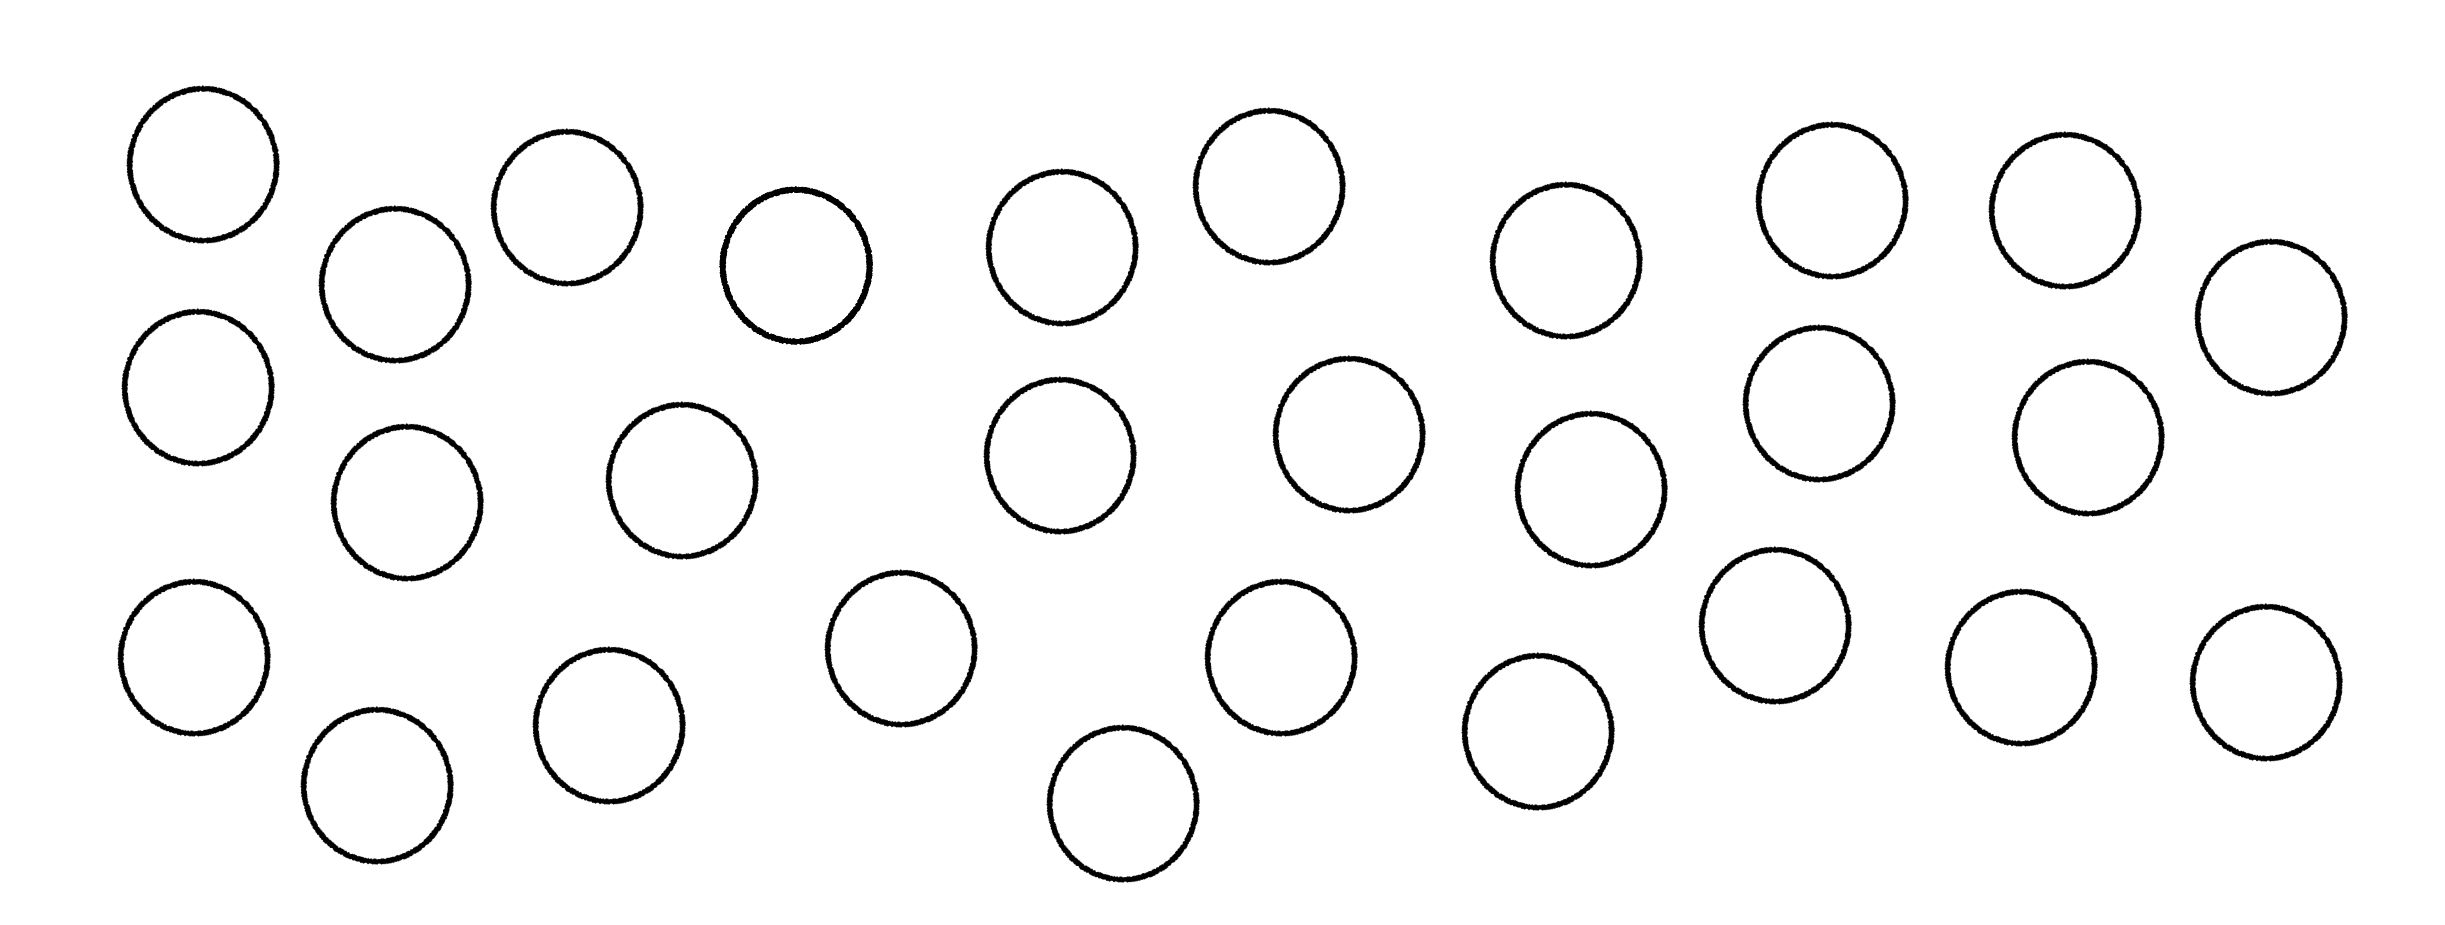
\includegraphics[width=\textheight ,
%    keepaspectratio]{surfacet1.jpg}}{test.mp4}

% \end{frame}
%%%%%%%%%%%%%%%%%%%%%%%%%%%%%%%%%%%%%%%%%%%%%%%%%%%%%%%%%%%%%%%%%%%

%%%%%%%%%%%%%%%%%%%%%%%%%%%%%%%%%%%%%%%%%%%%%%%%%%%%%%%%%%%%%%%%%%%
\newcounter{example}
 \setcounter{example}{1} 


 %%%%%%%%%%%%%%%%%%%%%%%%%%%%%%%%%%%%%%%%%%%%%%%%%%%%%%%%%%%%%%%



 \begin{frame}
  \frametitle{Example \theexample}

\begin{columns}[c]
\column{2in}  % slides are 3in high by 5in wide

\begin{figure}[h!]
  \begin{center}
    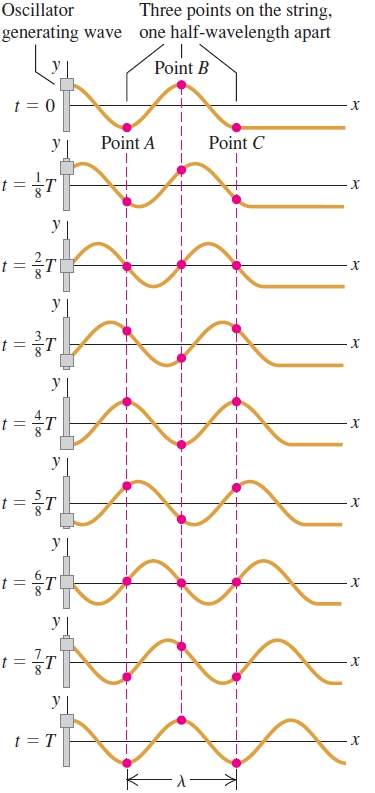
\includegraphics[height=3.in]{images4/EX1.jpg}
  \end{center}
\end{figure}



\column{2in}



(a) At which time is point A on the string moving upward with maximum speed?
(b) At which time does point B on the string have the greatest upward acceleration?
(c) At which time does point C on the string have a downward acceleration but an
upward velocity?



\end{columns}

\end{frame}
%%%%%%%%%%%%%%%%%%%%%%%%%%%%%%%%%%%%%%%%%%%%%%%%%
\stepcounter{example}

  \begin{frame}
    \frametitle{Example \theexample}

 One type of steel has density $\rho=7.8\times 10^3~kg/m^3$ and
will break if the tensile stress exceeds $7\times 10^8~N/m^2$. You want
to make a guitar string from $4.0 ~g$ of this type of steel. In use, the
guitar string must be able to withstand a tension of $900 ~N$ without
breaking. Your job is the following: (a) Determine the maximum
length and minimum radius the string can have. (b) Determine the
highest possible fundamental frequency of standing waves on this
string, if the entire length of the string is free to vibrate.

\end{frame}

  %%%%%%%%%%%%%%%%%%%%%%%%%%%%%%%%%%%%%%%%%%%%%%%%%%%%%%%%%%%%%%%

  \stepcounter{example}

  \begin{frame}
    \frametitle{Example \theexample}
    Two waves travel on the same string. Is it possible for them
    to have (a) different frequencies; (b) different wavelengths; (c) different
    speeds; (d) different amplitudes; (e) the same frequency but
    different wavelengths? Explain your reasoning.
  
  \end{frame}
  %%%%%%%%%%%%%%%%%%%%%%%%%%%%%%%%%%%%%%%%%%%%%%%%%%%%%%%%%%%%%%%
  \stepcounter{example}
  \begin{frame}
  \frametitle{Example \theexample}
  
  A tuning fork produces a steady $400~Hz$ tone. When this
  tuning fork is struck and held near a vibrating guitar string, twenty beats are counted
  in five seconds. What are the possible frequencies produced by the guitar string?
  
    \end{frame}
  
    %%%%%%%%%%%%%%%%%%%%%%%%%%%%%%%%%%%%%%%%%%%%%%%%%%%%%%%%%%%%%%%
    \stepcounter{example}
     
  \begin{frame}
    \frametitle{Example \theexample} 
    While a guitar string is vibrating,
you gently touch the midpoint of the string to ensure that the string does not vibrate at
that point. Which normal modes cannot be present on the string while you are touching it
in this way?
\end{frame}



%%%%%%%%%%%%%%%%%%%%%%%%%%%%%%%%%%%%%%%%%%%%%%%%%%%%%%%%%%%%%%%


  %%%%%%%%%%%%%%%%%%%%%%%%%%%%%%%%%%%%%%%%%%%%%%%%%%%%%%%%%%%%%%%
  \stepcounter{example}
  \begin{frame}
    \frametitle{Example \theexample} 


  When a massive aluminum sculpture is hung from a
steel wire, the fundamental frequency for transverse standing
waves on the wire is $250.0~ Hz$. The sculpture (but not the wire) is
then completely submerged in water. (a) What is the new fundamental
frequency?  (b) Why is it a good
approximation to treat the wire as being fixed at both ends?

\end{frame}

  %%%%%%%%%%%%%%%%%%%%%%%%%%%%%%%%%%%%%%%%%%%%%%%%%%%%%%%%%%%%%%%


\stepcounter{example}
\begin{frame}
  \frametitle{Example \theexample} 


  \begin{columns}[c]
    \column{2in}  % slides are 3in high by 5in wide
 
    \begin{figure}[h!]
      \begin{center}
        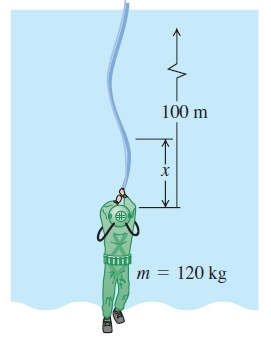
\includegraphics[height=2.in]{images4/15_84.jpg}
      \end{center}
    \end{figure}
    \column{2in}
 
 
    A deep-sea
    diver  jerks the end
    of the cable back and forth to
    send transverse waves up the
    cable as a signal to his companions
    in the boat. (a) What is the tension in the cable at its lower end,
    where it is attached to the diver?  (b)
    Calculate the tension in the cable a distance x above the diver.  (c)
    Find the time  required for the first signal to reach the surface.
  
    (The volume, the mass of the diver are known and the cross section of the cable too.)
  

    
    \end{columns}




  

\end{frame}



  %%%%%%%%%%%%%%%%%%%%%%%%%%%%%%%%%%%%%%%%%%%%%%%%%%%%%%%%%%%%%%%


  \stepcounter{example}
  \begin{frame}
    \frametitle{Example \theexample} 
  
  
    \begin{columns}[c]
      \column{2in}  % slides are 3in high by 5in wide
   
      \begin{figure}[h!]
        \begin{center}
          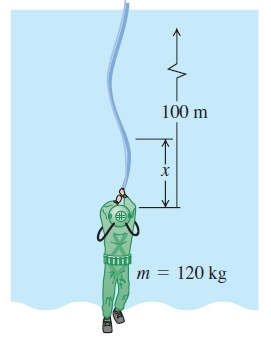
\includegraphics[height=2.in]{images4/15_84.jpg}
        \end{center}
      \end{figure}
      \column{2in}
   
   
 
  
      
      \end{columns}
  
  
  
  
    
  
  \end{frame}


    



%%%%%%%%%%%%%%%%%%%%%%%%%%%%%%%%%%%%%%%%%%%%%%%%%%%%%%%%%%%%%%%
 \end{document}
%%%%%%%%%%%%%%%%%%%%%%%%%%%%%%%%%%%%%%%%%%%%%%%%%%%%%%%%%%%%%%%